\documentclass{article}

\usepackage{graphicx}
\usepackage{tikz}
\usepackage{tikzsymbols}
\usetikzlibrary{calc,patterns,shapes.geometric}
\pagestyle{empty}
\usepackage[margin=0pt]{geometry}
\geometry{papersize={14in,12in}}

\def\centerarc[#1](#2)(#3:#4:#5){\draw[#1] ($(#2)+({#5*cos(#3)},{#5*sin(#3)})$) arc (#3:#4:#5);}

\begin{document}
	\begin{figure}
		\centering
		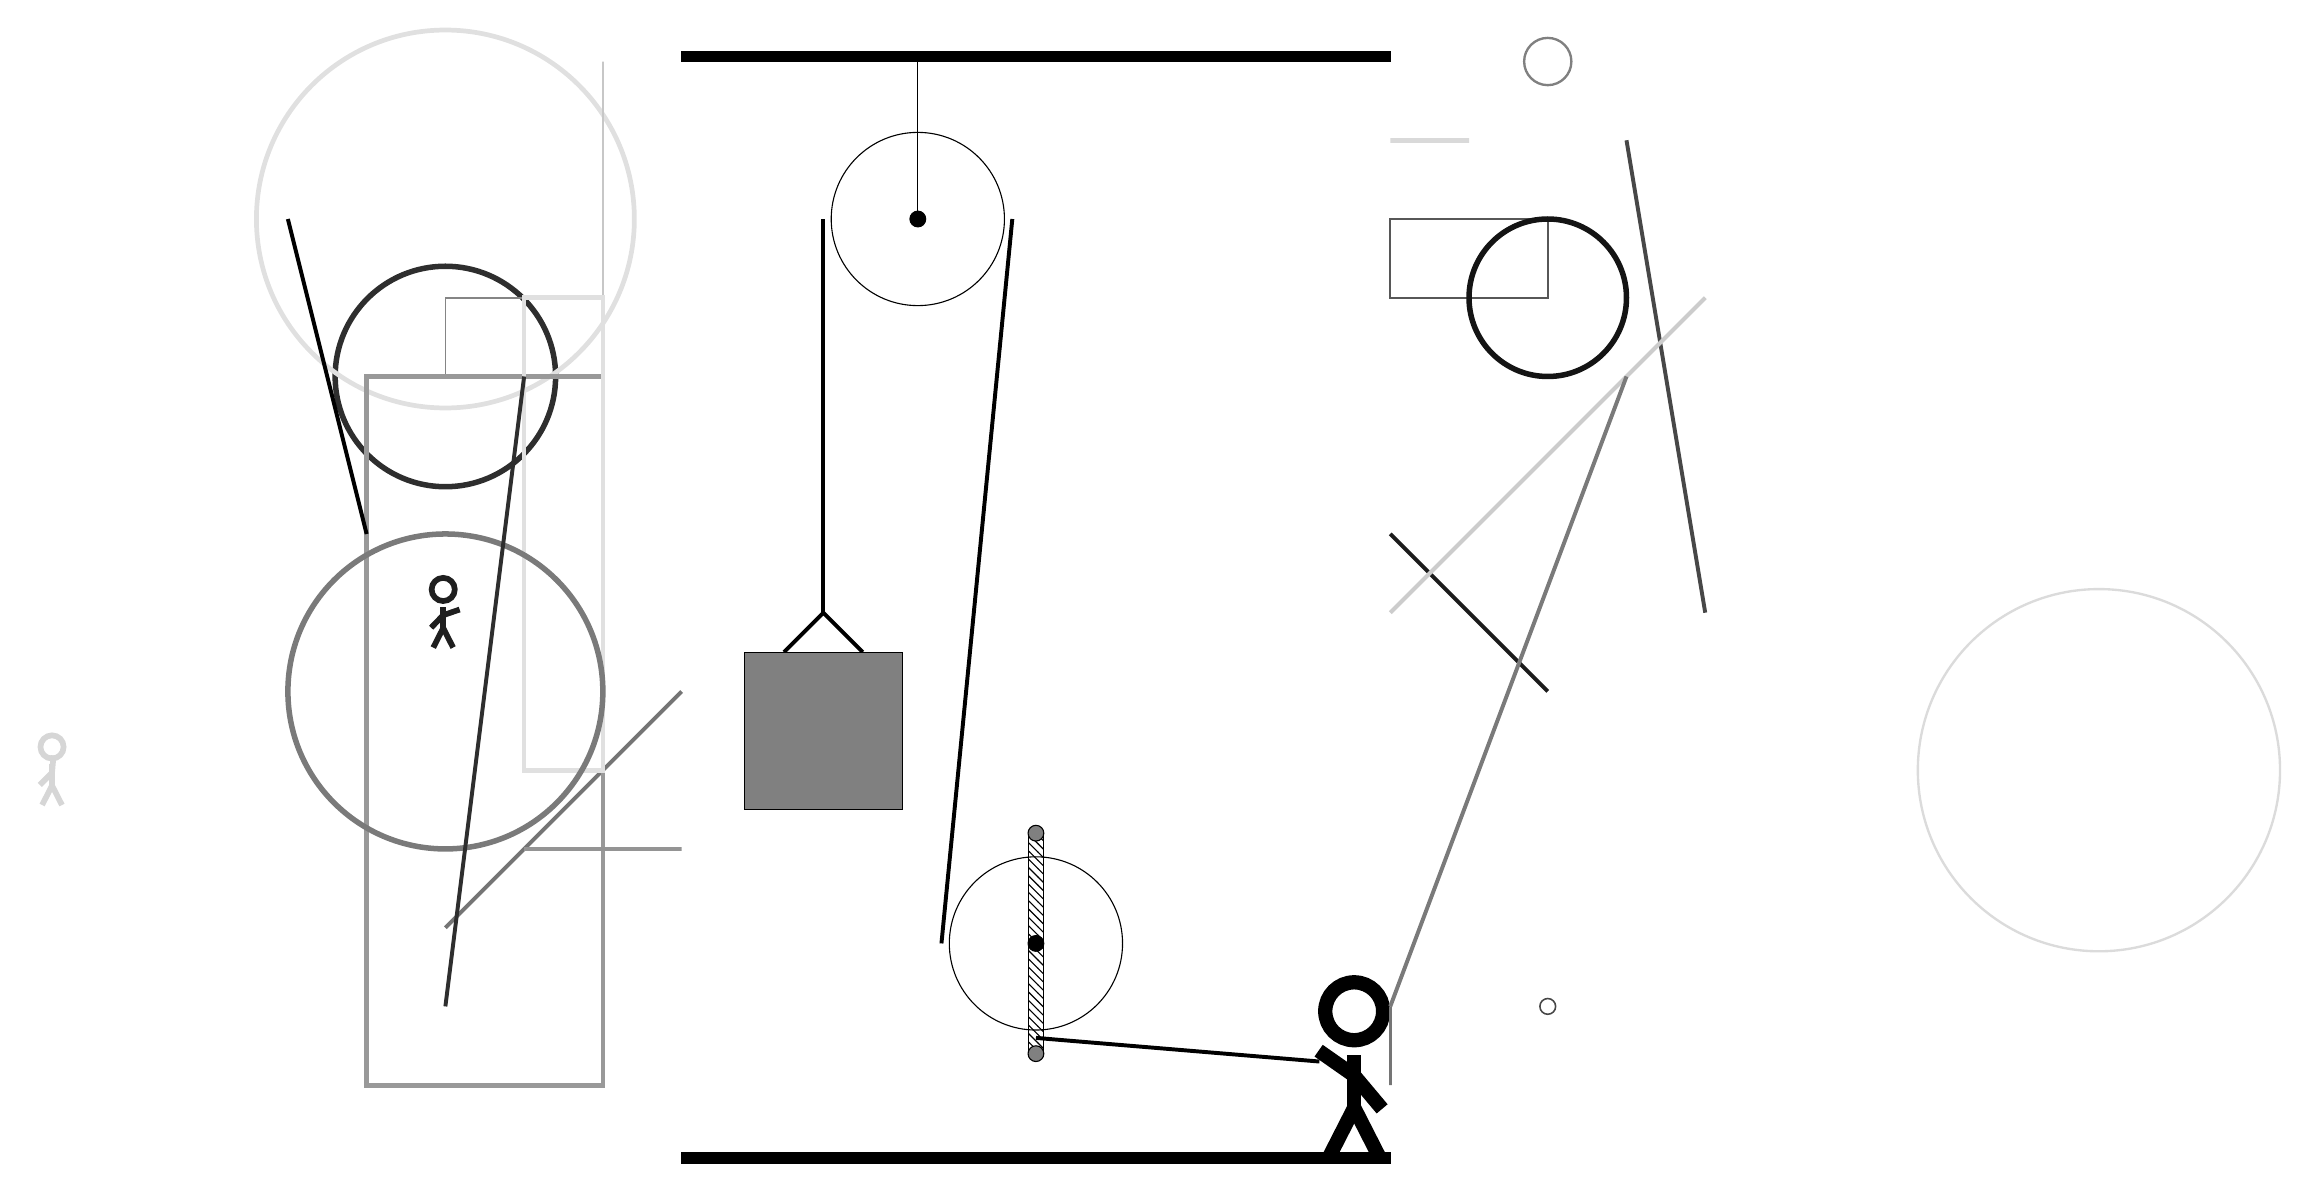
\begin{tikzpicture}
			%%%%% START %%%%%
			
			\draw[fill=black] (-2, 14) rectangle (7, 14.125);
			
			\draw (1, 12) circle (1.1);
			\draw[fill=black] (1, 12) circle (0.1);
			\draw (1, 14) -- (1, 12);
			
			\draw[fill=white](2.5, 2.8) circle (1.1);
			\draw[fill=black] (2.5, 2.8) circle (0.1);
			\draw[pattern=north west lines, pattern color=black] (2.4, 4.2) rectangle (2.6, 1.4);
			\draw[fill=black!50] (2.5, 4.2) circle (0.1);
			\draw[fill=black!50] (2.5, 1.4) circle (0.1);
			
			\draw[line width=0.5mm] (-0.7, 6.5) -- (-0.2, 7.0) -- (0.3, 6.5);
			\draw[fill=black!50] (-1.2, 6.5) rectangle (0.8, 4.5);
			
			\draw[line width=0.5mm] (-0.2, 12) -- (-0.2, 7.0);
			\centerarc[line width=0.5mm](1, 12)(0:180:1.2000000000000002);
			\draw[line width=0.5mm](2.2, 12) -- (1.3, 2.8);
			\centerarc[line width=0.5mm](2.5, 2.8)(180:270:1.2000000000000002);
			\draw[line width=0.5mm](2.5, 1.6) -- (6.1, 1.3);
			
			\node at (6.5, 1.2) {\Strichmaxerl[10][-35][-50]};
			
			\draw[line width=0.5mm, color=black!89](7, 8) -- (9, 6);
			
			\draw[line width=0.5mm, color=black!72](11, 7) -- (10, 13);
			\draw[line width=0.3mm, color=black!66] (7, 12) rectangle (9, 11);
			\draw [line width=0.7mm, color=black!82](-5, 10) circle (1.4);
			\draw[line width=0.2mm, color=black!48] (-3, 11) rectangle (-5, 10);
			\node[line width=0.2mm, color=black!88] at (-5, 7) {\Strichmaxerl[4][46][19]};
			\draw [line width=0.6mm, color=black!12](-5, 12) circle (2.4);
			\draw [line width=0.2mm, color=black!72](9, 2) circle (0.1);
			\draw[line width=0.2mm, color=black!22] (-3, 3) rectangle (-3, 14);
			\draw[line width=0.5mm, color=black!20](11, 11) -- (7, 7);
			\draw[line width=0.5mm, color=black!54](-5, 3) -- (-2, 6);
			\draw[line width=0.4mm, color=black!54] (7, 2) rectangle (7, 1);
			\draw[line width=0.3mm, color=black!90] (8, 7) rectangle (8, 7);
			
			\draw[line width=0.6mm, color=black!40] (-3, 1) rectangle (-6, 10);
			\draw[line width=0.5mm, color=black!52](10, 10) -- (7, 2);
			\draw[line width=0.6mm, color=black!12] (-3, 11) rectangle (-4, 5);
			
			\draw [line width=0.3mm, color=black!14](16, 5) circle (2.3);
			\draw[line width=0.5mm, color=black!100](-7, 12) -- (-6, 8);
			\node[line width=0.4mm, color=black!16] at (-10, 5) {\Strichmaxerl[4][45][85]};
			\draw[line width=0.6mm, color=black!15] (7, 13) rectangle (8, 13);
			\draw [line width=0.7mm, color=black!52](-5, 6) circle (2.0);
			
			\draw [line width=0.7mm, color=black!92](9, 11) circle (1.0);
			\draw[line width=0.6mm, color=black!42] (-2, 4) rectangle (-4, 4);
			\draw [line width=0.3mm, color=black!50](9, 14) circle (0.3);
			\draw[line width=0.5mm, color=black!82](-5, 2) -- (-4, 10);
			
			\draw[fill=black] (-2, 0) rectangle (7, 0.15);
			
			%%%%% END %%%%%
		\end{tikzpicture}
	\end{figure}	
\end{document}